{$\space$\par}
\vspace{0.5cm}
\justifying
\section*{{\bfseries \LARGE Questão 10 -} {\bfseries \large  Gaspar et al. (2003) publicaram dados de fotometria de estrelas do aglomerado NGC 2126. Esses dados estão no arquivo ngc2126.dat. Nesta análise, use apenas as componentes de movimento próprio (pmRA e pmDE). Nem todas as estrelas dessa tabela são membros reais de NGC 2126; a rigor, a maioria não deve ser. Para a análise, considere que toda estrela com movimento próprio total nulo provavelmente são estrelas mais distantes e não pertencem ao aglomerado. Entre as estrelas restantes, ainda deve haver algumas intrusas que se encontrem entre nós e o aglomerado; contudo, como o aglomerado se move de forma coesa, ele possui um valor bem marcado em pmRA e pmDE, e as estrelas intrusas serão outliers na distribuição dessas componentes. Use um método de densidade por kernel bidimensional para representar a densidade das estrelas no espaço de componentes do movimento próprio. Estime o movimento próprio mais provável desse aglomerado a partir das coordenadas (pmRA, pmDE) de maior densidade no seu gráfico. Anote-as no gráfico com o símbolo + vermelho, em tamanho cex = 2.5. }}

\vspace{0.8cm}

\begin{figure}[h]
    \centering
    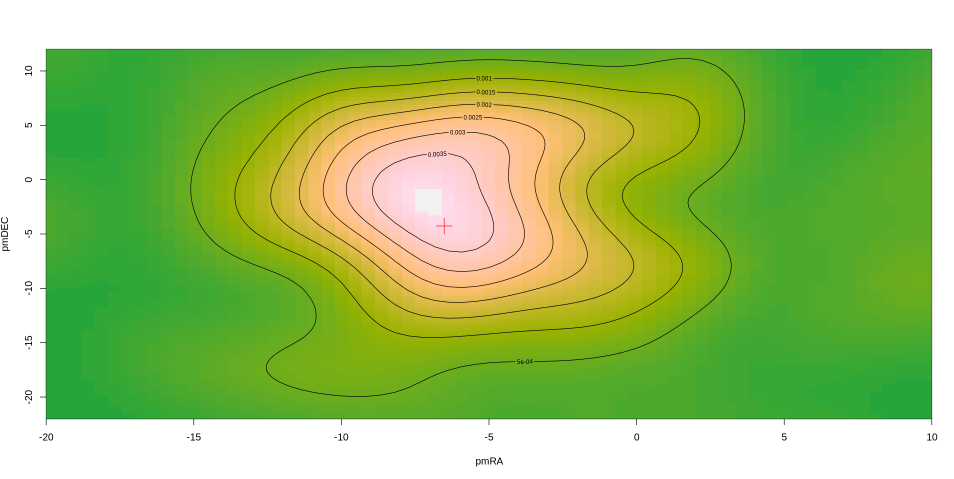
\includegraphics[width=0.8\linewidth]{Figuras/pmda_pmdec.png}
    \caption{Curvas de contorno juntas ao histograma 2D por kenerls das componentes RA e DEC do movimento próprio das estrelas do algomerado. A cruz vermelha indica o valor mais provável para o movimento próprio do aglomerado após separação de misturas.}
    \label{pmda_pmdec}
\end{figure}

\textcolor{red}{Para estimar a densidade bidimensional por kernel, utilizei o MASS:kde2d e o contour no kde para adicionar contornos. Como essa amostra contém outliers que não devem se mover da mesma maneira que o aglomerado, decidi utilizar o \texttt{mclust} para separar as possíveis misturas da amostra. Após realizar a separação em duas componentes gaussianas, o valor mais provável de movimento do aglomerado será o máximo de uma das gaussianas, ou seja, sua média, como mostrado na figura \ref{pmda_pmdec}.} 

\vspace{2em}

\begin{lstlisting}
    # Data
    ngc = read.table('/content/ngc2126.dat', sep='|', header=T)
    mask = sqrt(ngc$pmDE**2+ngc$pmRA**2)>0
    sample = ngc[mask,]

    # Splitting mixture
    model = Mclust(sample[,4:5],modelNames = 'VVV')
    model$parameters$mean

    ### output ###
    A matrix: 2 × 3 of type dbl
    pmRA	-6.517683	-4.151874	-0.9629393
    pmDE	-4.262831	4.439619	-13.9000586

    # Plotting
    kde = kde2d(sample$pmRA, sample$pmDE, n=200)
    image(kde, xlab='pmRA', ylab='pmDEC',col = hcl.colors(100, "terrain"), 
    xlim=c(-20,10),ylim=c(-22,12)) 
    
    #Cmap reference
    #https://www.rdocumentation.org/packages/graphics/versions/3.6.2/topics/image
    contour(kde,add=T)

    # Point
    points(model$parameters$mean[1,1],model$parameters$mean[2,1],pch=3,
    cex=2.5,col='red')
\end{lstlisting}

